\section{Open Search Tool: Pipeline Architecture and Implementation}

The Open Search Tool represents the information retrieval subsystem of Open Deep Search, responsible for transforming natural language queries into rich contextual information that enables factually grounded reasoning. This component implements a sophisticated three-stage pipeline that addresses fundamental challenges in web search including query understanding, result quality, and information depth. The design reflects careful consideration of trade-offs between retrieval coverage, computational cost, and result relevance. This section provides detailed examination of each pipeline stage, documenting implementation choices and their performance implications.

\subsection{Pipeline Overview and Information Flow}

The Open Search Tool operates as a sequential processing pipeline where each stage transforms and enriches the representation of information flowing through the system. A user query enters the pipeline as a simple text string expressing an information need. This query passes through three distinct processing stages, each addressing specific limitations of naive web search approaches.

The first stage performs query rephrasing, expanding the original query into multiple related formulations that capture different aspects of the underlying information need. This expansion addresses the semantic gap between how users express queries and the diverse ways relevant information appears in web documents. A single query formulation may miss relevant results that use different terminology, emphasize different aspects of the topic, or approach the subject from alternative perspectives. Query rephrasing generates diverse search formulations that collectively provide broader coverage of potentially relevant information.

The second stage executes retrieval operations using the rephrased queries against web search infrastructure. The system supports multiple search provider backends including the Serper.dev commercial API and self-hosted SearXNG instances. Each rephrased query generates a search request that returns a structured result set comprising titles, URLs, descriptive snippets, and metadata such as publication dates. The retrieval stage aggregates results across multiple queries, deduplicates entries appearing in multiple result sets, and organizes information for subsequent processing. The output from retrieval represents a collection of document pointers with associated metadata and brief content samples.

The third stage optionally performs augmentation that deepens the information available beyond search engine snippets. While retrieval provides pointers to relevant documents, augmentation fetches full content, extracts substantive passages, and identifies the portions most relevant to the original query. This processing involves web scraping to obtain complete document content, chunking that content into semantic units, generating embeddings that enable semantic similarity comparison, reranking chunks based on relevance to the query, and selecting top-scoring passages for inclusion in final context. The augmentation stage transforms shallow pointers into deep contextual information that supports comprehensive answer generation.

The output from the complete pipeline provides the reasoning agent with rich context comprising diverse information sources, relevant passages extracted from full documents, metadata enabling source evaluation, and structured organization facilitating information synthesis. This context serves as the foundation for subsequent reasoning, enabling the agent to formulate answers grounded in retrieved evidence rather than relying solely on parametric knowledge that may be outdated or incomplete.

The pipeline design reflects several important architectural principles. Each stage operates independently with well-defined inputs and outputs, enabling modular development and testing. The sequential flow ensures predictable execution order while the optional nature of augmentation provides flexibility to trade computational cost against information depth. The design accommodates different search providers without requiring changes to other pipeline stages, supporting both cloud-based and self-hosted deployment configurations. Error handling at each stage ensures graceful degradation where failures in later stages do not prevent the system from producing results based on earlier stage outputs.

\begin{figure}[htbp]
    \centering
    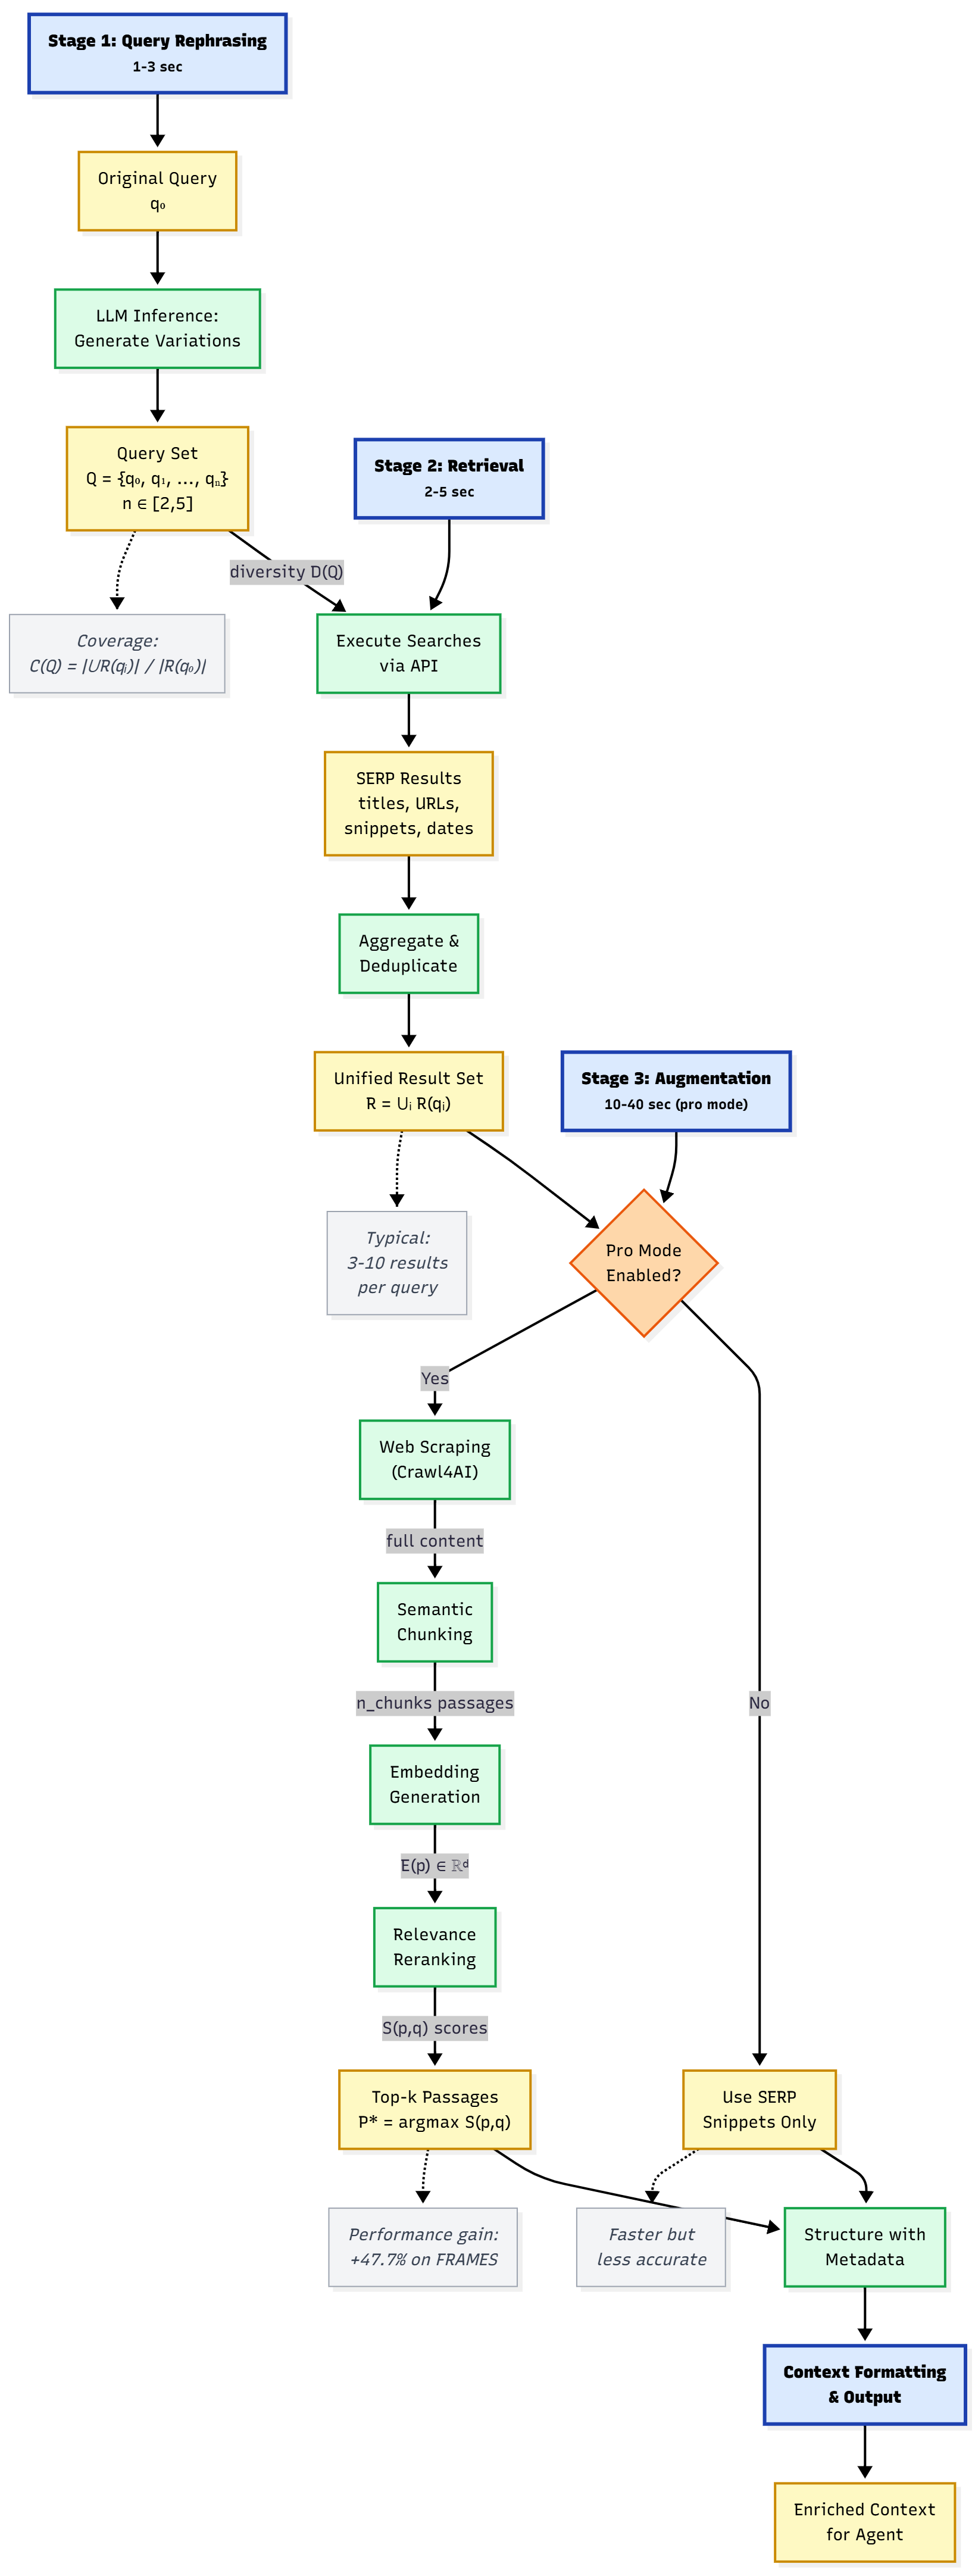
\includegraphics[width=0.5\linewidth]{figure2.png}
    \caption{Open Search Tool Pipeline: Three-Stage Information Flow. The pipeline progressively enriches query representation through (1) rephrasing for diversity, (2) retrieval across multiple formulations, and (3) optional deep augmentation. Pro mode augmentation provides 47.7\% accuracy improvement on FRAMES at the cost of 4-8$\times$ increased latency. Mathematical formulations show coverage gains ($C(Q)$}
    \label{fig:open_deep_search_architecture}
\end{figure}


\subsection{Query Rephrasing: Expanding Information Coverage}

The query rephrasing stage addresses a fundamental challenge in information retrieval where the vocabulary and structure of user queries often differ substantially from how relevant information appears in documents. This semantic gap causes relevant documents to be missed when they use terminology different from the query, emphasize different aspects of the topic, or frame information in ways that do not match the query structure. Query rephrasing mitigates this problem by generating multiple alternative formulations that collectively provide broader coverage of potentially relevant results.

The technical implementation leverages the base language model to generate rephrased queries. The system constructs a prompt that includes the original user query along with instructions to generate several alternative formulations that capture the same information need using different vocabulary, phrasing, and emphasis. The prompt explicitly requests queries that maintain the semantic intent of the original while exploring different ways the information might be expressed in documents. The language model generates between two and five alternative queries depending on the complexity and ambiguity of the original query.

Consider a concrete example where a user poses the query "How to make my Internet faster." This query contains implicit assumptions and underspecified aspects that could map to multiple distinct information needs. The rephrasing stage might generate alternatives including "How to make the WiFi signal stronger" that focuses on wireless connectivity, "How to increase bandwidth" that emphasizes network capacity, and "How to reduce latency" that targets response time. Each alternative query potentially retrieves documents that would be missed by the others, collectively providing more comprehensive coverage of information relevant to improving internet performance.

The rephrasing strategy employs several techniques to ensure diversity and relevance of generated queries. Vocabulary expansion replaces terms with synonyms and related concepts, transforming "Internet" to "network connection" or "online access." Perspective shifting reformulates queries from different angles, changing "how to make faster" to "what causes slow speed" that inverts the framing. Specificity variation generates both more specific queries that add details and more general queries that broaden scope. Implicit concept extraction identifies unstated assumptions in the original query and makes them explicit in alternatives.

The query rephrasing mechanism provides measurable benefits to overall system performance. Empirical evaluation demonstrates that rephrasing substantially improves retrieval diversity, measured by the number of unique relevant documents found across all generated queries compared to using only the original formulation. The expanded query set increases coverage of relevant information sources, particularly for ambiguous queries where multiple valid interpretations exist. The diversity benefit proves most valuable for complex queries requiring synthesis across multiple perspectives, while providing marginal gains for simple factual lookups where the original query formulation suffices.

\newpage

The mathematical formulation of query diversity can be expressed as follows. Given an original query $q_0$, the system generates a set of reformulations:

\begin{equation}
Q = \{q_0, q_1, q_2, \ldots, q_n\} \quad \text{where } n \in [2,5]
\label{eq:query_set}
\end{equation}

The coverage metric measuring information retrieval improvement is defined as:

\begin{equation}
C(Q) = \frac{\left|\bigcup_{i=0}^{n} R(q_i)\right|}{|R(q_0)|}
\label{eq:coverage}
\end{equation}

where $R(q)$ denotes the set of relevant documents retrieved by query $q$. The diversity score across reformulations is computed as:

\begin{equation}
D(Q) = \frac{1}{n^2} \sum_{i \neq j} d(q_i, q_j)
\label{eq:diversity}
\end{equation}

where $d(\cdot, \cdot)$ represents the semantic distance between query pairs, typically measured using embedding-based cosine distance.

The implementation includes several refinements that improve practical effectiveness. The system maintains the original query in the set of queries to execute, ensuring that the user's specific formulation receives consideration alongside generated alternatives. Rephrased queries undergo filtering to remove duplicates and near-duplicates that would waste resources on redundant searches. The language model receives guidance on maintaining query length within reasonable bounds, avoiding both excessively terse formulations that lose important context and overly verbose formulations that may confuse search engines. Temperature settings control the diversity of generated alternatives, balancing between conservative rephrasing that stays close to the original and aggressive rephrasing that explores more distant reformulations.

Certain limitations affect the query rephrasing approach. The quality of generated alternatives depends heavily on the capabilities of the base language model, with more capable models producing more useful reformulations. The rephrasing process adds latency by requiring an additional language model inference call before search begins, typically adding one to three seconds depending on model speed. The approach generates modest additional search API costs by executing multiple queries instead of one, though this cost remains relatively small compared to the value of improved coverage. The technique provides greatest benefit for ambiguous or complex queries, offering diminishing returns for simple factual lookups that have clear, unambiguous formulations.

Despite these limitations, query rephrasing represents a critical component of the Open Search Tool that substantially improves retrieval effectiveness. The relatively modest computational cost proves worthwhile given the significant improvements in coverage and diversity of retrieved information. The modular implementation allows the rephrasing strategy to evolve independently as better techniques emerge without requiring changes to other pipeline stages.

\subsection{Retrieval: Search Provider Integration and Result Collection}

The retrieval stage executes search operations using rephrased queries against web search infrastructure, collecting structured result sets that point to potentially relevant documents. This stage implements abstraction over multiple search provider backends, enabling flexible deployment configurations that balance cost, privacy, and search quality considerations.

The Open Search Tool supports two primary search provider options with distinct characteristics and trade-offs. The Serper.dev integration provides access to Google search results through a commercial API, offering high-quality search powered by Google's comprehensive index and sophisticated ranking algorithms. The service provides a free tier with 2,500 search credits, making it accessible for development and moderate-scale deployment. Beyond the free tier, usage incurs costs based on search volume. The integration requires only an API key configured through environment variables, offering minimal setup complexity. The Serper.dev option proves well-suited for deployments prioritizing search quality and rapid implementation over cost optimization at scale.

The SearXNG integration provides an alternative path using open-source metasearch infrastructure. SearXNG operates as a privacy-respecting metasearch engine that aggregates results from multiple search backends while protecting user privacy. Users can either deploy their own SearXNG instance for complete control or connect to public community-run instances. Self-hosted deployment requires infrastructure to run the SearXNG service but eliminates per-search API costs, providing cost advantages at scale. The integration accepts both instance URL and optional API key for authenticated access to protected instances. The SearXNG option suits deployments prioritizing cost control, privacy preservation, or independence from commercial search providers.

The retrieval process follows a consistent pattern regardless of which search provider is configured. The system iterates through the collection of queries including both the original and rephrased variants, executing a search request for each query. Each search returns a structured result set containing multiple entries. For each entry, the system extracts several pieces of metadata. The title provides a brief headline describing the document. The URL identifies the document location for potential subsequent access. The description snippet offers a brief excerpt showing how the document relates to the query. The publication date when available indicates document freshness and relevance to time-sensitive queries.

The retrieval stage implements several processing steps to organize and deduplicate collected results. As results arrive from multiple searches, the system identifies duplicates where the same document appears in multiple result sets, typically occurring when different query formulations retrieve overlapping relevant documents. Deduplication prevents redundant processing of the same content in later stages. The system preserves the highest-ranked occurrence of each document, reflecting the assumption that higher ranking indicates greater relevance. Result aggregation combines entries from all searches into a unified collection suitable for subsequent processing.

The metadata collected during retrieval serves multiple important purposes beyond simply identifying documents. Publication dates enable temporal filtering where the reasoning agent can prioritize recent information for queries requiring current data. URL domains provide signals about source credibility, with certain top-level domains like government and educational institutions carrying higher authority for factual information. Description snippets offer preview content that enables quick relevance assessment without requiring full document fetching. Title text provides concise summaries useful for understanding document focus.

The implementation includes several technical considerations that affect practical deployment. Search API rate limiting requires careful management to avoid exceeding provider quotas, particularly when executing multiple rephrased queries per user request. The system implements rate limiting logic and retry mechanisms to handle temporary failures gracefully. Error handling addresses various failure modes including network timeouts, API authentication errors, and malformed responses. Fallback logic ensures that failures retrieving results for some queries do not prevent the system from using successfully retrieved results from other queries.

The retrieval stage exposes configuration parameters that enable tuning for specific deployment requirements. The number of results to retrieve per query can be adjusted based on whether thoroughness or speed is prioritized. The maximum time to wait for search responses allows control over worst-case latency when search providers experience slow responses. Provider selection enables switching between Serper and SearXNG based on deployment preferences. Result filtering can apply domain restrictions to exclude or specifically include certain website categories.

The abstraction over multiple search providers provides important benefits for the Open Deep Search ecosystem. Users can select providers based on their specific constraints without requiring system modifications. Development can proceed using the simpler Serper integration while production deployment switches to self-hosted SearXNG for cost and privacy benefits. The architecture remains open to additional search provider implementations as new options emerge or specialized search engines become available for particular domains.

\subsection{Augmentation: Deep Content Extraction and Semantic Reranking}

The augmentation stage represents the most computationally intensive component of the Open Search Tool pipeline, transforming shallow document pointers into deep contextual information through web scraping, content extraction, and semantic relevance assessment. This processing proves essential for complex multi-hop queries requiring synthesis across multiple sources, while remaining optional for simpler queries where search engine snippets provide sufficient context.

The augmentation process begins with web scraping to obtain full content from documents identified during retrieval. The system leverages Crawl4AI, a sophisticated web crawling library designed specifically for extracting clean content from modern web pages. Contemporary websites present substantial challenges for content extraction including Java  Script rendered content that requires execution to access, complex layouts with navigation and advertising that obscure main content, and anti-scraping measures designed to prevent automated access. Crawl4AI addresses these challenges through headless browser automation that executes JavaScript, content extraction algorithms that identify main text while filtering boilerplate, and polite crawling behavior that respects robots.txt directives and implements rate limiting.

The scraping process operates on a configurable subset of top-ranked URLs from the retrieval results, typically processing between three and ten documents depending on the thoroughness versus latency trade-off selected for the deployment. Each URL triggers an asynchronous fetch operation that retrieves the page, executes any required JavaScript, extracts textual content, and returns cleaned text suitable for subsequent processing. The system implements error handling for common failure modes including pages that no longer exist, content behind paywalls or authentication requirements, and malformed HTML that resists parsing. Failed fetches do not halt the pipeline but simply result in fewer documents available for subsequent processing.

Following successful content extraction, the augmentation stage performs passage chunking to break lengthy documents into semantic units suitable for relevance assessment. Native web pages often contain thousands or tens of thousands of words spanning multiple topics, only portions of which relate to the query. Processing entire documents as single units would make relevance assessment coarse and potentially miss relevant passages embedded within largely irrelevant content. Chunking divides documents into passages of manageable length, typically ranging from 200 to 500 words, creating discrete units that can be individually assessed for relevance.

The chunking strategy attempts to preserve semantic coherence by identifying natural breakpoints in document structure. The algorithm considers paragraph boundaries, section headings, and other structural markers that indicate topic transitions. This semantic chunking produces more coherent passages than simple fixed-length splitting that might divide sentences or paragraphs. Each chunk maintains association with source metadata including the document URL, title, and position within the original document, enabling provenance tracking for included passages.

The embedding generation phase transforms textual chunks into dense vector representations that enable semantic similarity comparison. The system generates embeddings using either cloud-based services like Jina AI or self-hosted infrastructure through Infinity Embeddings depending on deployment configuration. The embedding model transforms each chunk into a high-dimensional vector, typically 768 or 1,024 dimensions, where semantically similar text produces vectors close together in the embedding space. This mathematical representation enables quantitative measurement of how well each passage matches the query.

The reranking phase leverages embeddings to assess relevance of each chunk to the original user query. The system generates an embedding for the query using the same model used for passage embeddings, ensuring compatibility in the vector space. For each chunk, the system computes cosine similarity between the chunk embedding and query embedding, producing a relevance score between zero and one where higher values indicate greater semantic alignment. 

The passage relevance scoring mechanism can be formalized mathematically. For a given passage $p_i$ and query $q$, the relevance score is computed as:

\begin{equation}
S(p_i, q) = \cos(E(p_i), E(q)) = \frac{E(p_i) \cdot E(q)}{\|E(p_i)\| \|E(q)\|}
\label{eq:relevance_score}
\end{equation}

where $E: \text{text} \to \mathbb{R}^d$ is the embedding function mapping text to a $d$-dimensional vector space, with $d \in \{768, 1024\}$ depending on the model architecture.

The top-$k$ passage selection optimizes for both relevance and source diversity:

\begin{equation}
P^* = \argmax_{\substack{P \subset \text{Passages} \\ |P| = k}} \sum_{p \in P} S(p, q) \cdot w(\text{source}(p))
\label{eq:topk_selection}
\end{equation}

where $w(\cdot)$ assigns authority weights to different information sources, with higher weights for government domains (.gov), educational institutions (.edu), and peer-reviewed publications.

The system sorts all chunks by relevance score, identifying the passages most closely matching the query intent.

The final selection step chooses the top-k highest-scoring passages for inclusion in the context provided to the reasoning agent. The value of k represents a trade-off between context richness and computational efficiency, typically ranging from five to twenty passages depending on the query complexity and available model context window. The selected passages span multiple source documents when multiple documents contain relevant information, providing diverse perspectives and increasing confidence through cross-source verification. The system preserves source attribution for each passage, enabling the reasoning agent to cite specific sources when formulating answers.

The augmentation process provides dramatic performance improvements for certain query categories. Empirical evaluation on the FRAMES benchmark demonstrates that enabling augmentation improves accuracy from 27.6 percent to 75.3 percent when using Open Deep Search version 2 with DeepSeek-R1, a gain of 47.7 percentage points. This substantial improvement reflects the value of deep content access for complex multi-hop queries requiring synthesis of information scattered across multiple documents. Search engine snippets alone prove insufficient for these queries, as the relevant information often appears in passages beyond what snippets capture.

The computational cost of augmentation manifests across several dimensions. Web scraping adds latency through multiple HTTP requests, typically requiring one to five seconds per page depending on page complexity and network conditions. Processing multiple pages sequentially can extend total scraping time to fifteen seconds or more, though parallel fetching can reduce this substantially. Embedding generation requires neural network inference for potentially dozens or hundreds of chunks, adding several seconds depending on whether cloud APIs or local inference is used. Reranking computation remains relatively lightweight as it involves only vector similarity calculations.

Several implementation refinements improve the practical effectiveness of augmentation. Caching of scraped content reduces redundant fetching when the same URLs appear across multiple queries, particularly valuable for popular reference sources like Wikipedia that appear frequently in search results. Embedding caching stores generated vectors for passages, enabling reuse when the same content appears in different contexts. Parallel processing executes web scraping for multiple URLs concurrently rather than sequentially, substantially reducing total latency. Adaptive depth control adjusts the number of URLs to scrape based on query complexity detection, processing more documents for complex queries while limiting scraping for simple lookups.

The augmentation stage exposes several configuration parameters enabling tuning for specific requirements. The maximum number of URLs to scrape controls thoroughness versus latency trade-offs. The target chunk size affects granularity of relevance assessment. The number of top passages to include determines context richness. The choice between Jina AI and Infinity for reranking balances convenience against cost and privacy. The minimum relevance threshold filters out marginally relevant passages that might introduce noise.

Certain specialized handling improves effectiveness for common website types. Wikipedia pages receive special parsing that preserves article structure and extracts key summary information. ArXiv papers undergo processing that identifies and emphasizes abstract and conclusion sections. PubMed entries receive handling tailored to medical literature structure. These domain-specific optimizations improve the quality of extracted content for frequently encountered information sources.

The augmentation architecture maintains extensibility for future enhancements. The modular design enables replacement of individual components such as the web scraping library, embedding model, or reranking algorithm without affecting other stages. This flexibility supports ongoing improvement as better techniques emerge for each aspect of the augmentation pipeline. The abstraction over embedding providers enables easy adoption of new state-of-the-art embedding models as they become available.

\subsection{Context Formatting and Source Attribution}

The final responsibility of the Open Search Tool involves formatting retrieved and augmented information into structured context suitable for consumption by reasoning agents. The formatting strategy draws inspiration from the FreshPrompt methodology that demonstrated the value of rich metadata in improving language model reasoning over retrieved information.

The context structure organizes information hierarchically with clear delineation between different sources and passages. Each source document receives a distinct section containing its metadata and associated content. The metadata block includes the document title providing a concise summary, the source URL enabling verification and further investigation, the publication date when available indicating information freshness, and the description snippet from search results offering context. Following metadata, the system includes relevant passages extracted during augmentation or the description snippet if augmentation was not performed.

The formatting employs explicit markers to help reasoning agents parse and utilize the information effectively. Source sections begin with clear headers identifying them as distinct documents. Passage boundaries use consistent delimiters that enable the agent to distinguish between content from different portions of documents. Attribution markers link passages to their source documents, maintaining provenance throughout the reasoning process. Metadata fields use structured formats that facilitate programmatic extraction when needed.

The context formatting implements several strategies to improve reasoning agent effectiveness. Source prioritization places more authoritative or recent sources earlier in the context, taking advantage of primacy effects where early information receives greater weight in language model reasoning. Relevance ordering arranges passages by their reranking scores, ensuring the most relevant information appears prominently. Length management truncates or summarizes excessively long passages to fit within available context windows while preserving key information. Redundancy reduction identifies and consolidates highly similar passages that would waste context capacity.

Special formatting applies to sources from different domains based on their characteristics and typical usage patterns. Government sources receive markers indicating their authoritative status for factual claims. Educational institution sources (.edu domains) get highlighted given their generally high credibility. Peer-reviewed publications receive special formatting that emphasizes their scholarly nature. News sources include publication date prominently given the time-sensitivity of news information. User-generated content platforms receive markers indicating the need for careful verification.

The system implements source diversity promotion that ensures the selected passages span multiple independent sources when possible. Relying on a single source increases vulnerability to errors or biases in that source. Multiple sources enable cross-verification where claims appearing in multiple independent sources gain confidence. The diversity promotion mechanism tracks source URLs and attempts to select passages from different domains rather than concentrating on a single highly-relevant website.

The context formatting stage produces output consumed by reasoning agents in different ways depending on the agent framework. ReAct agents receive context formatted with clear structure that facilitates parsing during the observation phase following search actions. CodeAct agents receive context that can be easily manipulated programmatically within generated Python code. Both frameworks benefit from consistent formatting that reduces the parsing and interpretation complexity facing the language model.

The implementation includes comprehensive logging of the complete search pipeline for debugging and analysis purposes. Logs capture the original query, all rephrased query variants, raw search results from each query, URLs selected for scraping, successfully scraped content, generated embeddings, reranking scores, selected passages, and final formatted context. This detailed logging proves invaluable for diagnosing failures, understanding system behavior, and identifying opportunities for improvement. Production deployments can adjust logging verbosity based on operational requirements.

The Open Search Tool concludes by returning structured context to the reasoning agent that invoked it. This context contains rich information gathered from diverse sources, processed to emphasize relevant passages, annotated with metadata enabling source evaluation, and formatted for effective reasoning agent consumption. The tool operates as a self-contained module that encapsulates all complexity of web search, content extraction, and relevance assessment, presenting a clean interface to reasoning components that simply invoke the tool and receive structured results.

\subsection{Performance Characteristics and Optimization}

The Open Search Tool exhibits performance characteristics that vary substantially based on configuration choices and operational mode selection. Understanding these characteristics enables informed decisions about deployment configurations and appropriate trade-offs for specific use cases.

Latency represents the primary performance dimension users experience directly. In default mode without augmentation, the Open Search Tool typically completes in three to eight seconds depending on the number of rephrased queries and search API response time. Query rephrasing consumes one to three seconds for language model inference. Each search request adds 200 to 500 milliseconds depending on the search provider, with multiple queries executing sequentially extending this time. Result aggregation and deduplication add negligible overhead.

In pro mode with augmentation enabled, latency extends substantially. Web scraping adds one to five seconds per page depending on page complexity, network latency, and whether pages require JavaScript execution. Processing ten pages sequentially extends total scraping time to fifteen seconds or more in worst cases. Embedding generation adds 500 milliseconds to two seconds depending on whether cloud APIs or local inference is used and how many chunks require processing. Reranking computation adds 200 to 800 milliseconds for scoring all chunks. Total pro mode latency typically ranges from fifteen to sixty seconds with high variance based on query characteristics.

Several optimization techniques substantially reduce latency in practical deployments. Parallel web scraping executes fetches for multiple URLs concurrently rather than sequentially, reducing scraping time by 60 to 70 percent when processing ten pages. Embedding batch processing generates vectors for multiple chunks in a single inference call, improving throughput over per-chunk inference. Result caching stores search results with time-to-live parameters, eliminating retrieval latency for repeated queries. Content caching stores scraped webpage content, avoiding redundant fetches for popular sources. Embedding caching stores generated vectors persistently, enabling reuse across queries.

Computational cost comprises multiple components with different scaling characteristics. 
Search API costs depend on the number of queries executed, typically ranging from 
\$0.01 to \$0.03 per search. 
Query rephrasing requires language model inference costing 
\$0.002 to \$0.01 depending on the model used and the number of tokens processed. 
Augmentation adds embedding generation costs of 
\$0.01 to \$0.03 when using cloud services like Jina AI, 
or local compute costs when self-hosting. 
Web scraping incurs bandwidth costs that remain negligible for most deployments. 
Total per-query costs range from \$0.005 to \$0.03 depending on configuration 
and operational mode.

Self-hosted deployments shift the cost structure from per-query API charges to fixed infrastructure costs. Running a SearXNG instance requires a modest virtual machine costing 
\$20 to \$50 monthly. Self-hosted embedding generation through Infinity requires GPU infrastructure that may already exist for hosting language models, adding marginal cost. At scale, self-hosting substantially reduces per-query costs while requiring operational expertise to maintain infrastructure.

Search quality represents another critical performance dimension that proves more difficult to quantify than latency or cost. The choice of search provider affects result relevance, with Google-backed options like Serper generally providing higher quality than alternatives. Query rephrasing improves search quality by increasing coverage and diversity of retrieved results, with benefits proportional to query ambiguity. Augmentation dramatically improves quality for complex queries by enabling access to detailed information beyond snippets, though it provides minimal benefit for simple factual lookups where snippets suffice.

The Open Search Tool exposes several tuning parameters that enable users to navigate performance trade-offs based on their priorities. The number of rephrased queries controls coverage versus latency and cost. The number of search results retrieved per query affects thoroughness. The number of URLs to scrape during augmentation determines information depth. The number of passages to include in final context balances richness against context window consumption. Temperature parameters control diversity in query rephrasing. Timeout values limit worst-case latency for misbehaving components.

Certain query characteristics significantly affect performance. Simple factual queries with unambiguous answers execute quickly and benefit little from augmentation. Complex multi-hop queries requiring synthesis across sources take substantially longer but benefit dramatically from augmentation. Queries about recent events encounter fresher information in search results. Queries about obscure topics may struggle to find relevant sources. The system adapts to query characteristics through mechanisms like adaptive mode selection, dynamic rephrasing based on complexity, and relevance threshold adjustment.

The performance profile suggests different deployment strategies for different use cases. Latency-sensitive interactive applications should use default mode, minimize rephrasing, implement aggressive caching, and consider response streaming to provide incremental results. Accuracy-focused research applications should use pro mode, maximize augmentation depth, prefer self-hosted infrastructure to eliminate API latency, and accept longer response times. Cost-sensitive deployments should self-host where possible, implement comprehensive caching, use smaller language models for rephrasing, and carefully tune augmentation parameters.

Monitoring and observability prove essential for production deployments to understand actual performance characteristics and identify optimization opportunities. Key metrics include query latency at various percentiles, cost per query averaged over time windows, cache hit rates for different caching layers, search API response times, web scraping success rates, and embedding generation throughput. These metrics enable data-driven optimization and capacity planning.

The Open Search Tool achieves its performance characteristics through careful engineering and thoughtful architectural decisions. While latency exceeds that of proprietary alternatives optimized at massive scale, the performance proves acceptable for many use cases while providing the transparency, customizability, and cost advantages that motivate open-source adoption. Ongoing optimization efforts continue to improve performance as the codebase matures and as better underlying components become available.
